%\iffalse
\let\negmedspace\undefined
\let\negthickspace\undefined
\documentclass[journal,12pt,twocolumn]{IEEEtran}
\usepackage{cite}
\usepackage{amsmath,amssymb,amsfonts,amsthm}
\usepackage{algorithmic}
\usepackage{graphicx}
\usepackage{textcomp}
\usepackage{xcolor}
\usepackage{txfonts}
\usepackage{listings}
\usepackage{enumitem}
\usepackage{mathtools}
\usepackage{gensymb}
\usepackage{comment}
\usepackage[breaklinks=true]{hyperref}
\usepackage{tkz-euclide} 
\usepackage{listings}
\usepackage{gvv}                                        
\def\inputGnumericTable{}                                 
\usepackage[latin1]{inputenc}                                
\usepackage{color}                                            
\usepackage{array}                                            
\usepackage{longtable}                                       
\usepackage{calc}                                             
\usepackage{multirow}                                         
\usepackage{hhline}                                           
\usepackage{ifthen}                                           
\usepackage{lscape}

\newtheorem{theorem}{Theorem}[section]
\newtheorem{problem}{Problem}
\newtheorem{proposition}{Proposition}[section]
\newtheorem{lemma}{Lemma}[section]
\newtheorem{corollary}[theorem]{Corollary}
\newtheorem{example}{Example}[section]
\newtheorem{definition}[problem]{Definition}
\newcommand{\BEQA}{\begin{eqnarray}}
\newcommand{\EEQA}{\end{eqnarray}}
\newcommand{\define}{\stackrel{\triangle}{=}}
\theoremstyle{remark}
\newtheorem{rem}{Remark}
\begin{document}
\bibliographystyle{IEEEtran}
\vspace{3cm}
\title{\textbf{11.9.3}}
\author{EE23BTECH11053-R.Rahul$^{*}$% <-this % stops a space
}
\maketitle
\newpage
\bigskip

\textbf{QUESTION:}\\
1.How many terms of G.P.$3$,$3^2$,$3^3$, \ldots are needed to give the sum $120$ ?\\

\textbf{SOLUTION:}\\
\vspace{-0.25cm}


\begin{table}[h]
  \centering
  \begin{tabular}{|c|c|c|c|c|c| }
    \hline
    \(n\) & \(x_1(n)\)& \(x_2(n)\) & \(x_3(n)\) & \(x_4(n)\) & \(x_5(n)\) \\
    \hline
    0 & 2  & 18 &  5  &  -4  &  53  \\
    1 & 14 & 13 & $6\frac{1}{2}$ & -2 & 38 \\
    2 & 26 & 8 & 8 & 0 & 23 \\
    3 & 38 & 3 & $9\frac{1}{2}$ & 2 & 8 \\
    4 & 50 & -2 & 11 & 4 & -7 \\
    5 & 62 & -7 & $12\frac{1}{2}$ & 6 & -22 \\
    \hline
  \end{tabular}
  \caption{first three terms of AP series}
  \label{tab:xn}
\end{table}



\begin{center}
    
\begin{align}
      X(z)&=\frac{x(0)}{1-rz^{-1}} \qquad |z|>|r|\\
      &=\frac{3}{1-3z^{-1}}\\
      U(z)&=\frac{1}{1-z^{-1}} \qquad |z|>1\\
      y(n)&= x(n)*u(n)\\
      Y(z)&=X(z)U(z)\\
&=\brak{ \frac{3}{1-3z^{-1}}}\brak{\frac{1}{1-z^{-1}}}\quad|z| > 3 \end{align}
\end{center}
Using Contour integration\\
\begin{center}
 \begin{align}
   y(n)&=\frac{1}{2\pi j}\oint_C \frac{3 z^2}{(z-1)(z-3)}z^{n-1} dz\\
   &=\frac{1}{2 \pi j}\oint_C \frac{3}{2} \brak{\frac{1}{z-3} - \frac{1}{z-1}z^{n+1}}dz\\
   120&= \frac{3}{2}(3^{n}- 1)\\
   n&=4
 \end{align}
\end{center}

\begin{figure}[h]
  
  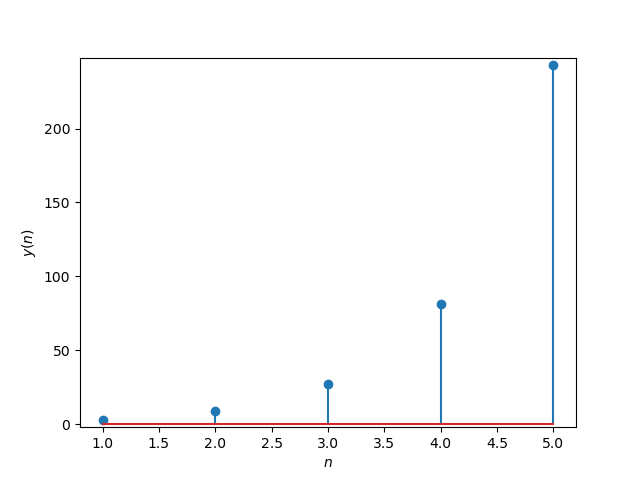
\includegraphics[width=\columnwidth]{figs/graph.png}
  \caption{Stem plot of y(n)}
  \label{fig:your_label}
\end{figure}



\end{document}
